%4
\section{Konkrete Architektur}
%4.1 Server Software
\subsection{\textit{ServerSoftware}}
\begin{figure}[H]
\centering
\includegraphics[width=0.7\textwidth]{img/51}
\caption{Komponentendiagramm für den \emph{Server}}
\label{KomponentendiagrammKonkretServer}
\end{figure}
Abbildung \ref{KomponentendiagrammKonkretServer} zeigt das konkrete Komponentendiagramm für die Komponente \emph{Server}. Die \emph{ServerSoftware} tätigt in der aktuellen nullten Ausbaustufe direkt Aufrufe an den \textit{Robot}, 
um den besten \textit{Robot} für eine \textit{Destination} zu ermitteln und einem \textit{Robot} eine \textit{Destination} zuzuweisen.

%4.2 Robot Software
\subsection{\textit{RobotSoftware}}
\begin{figure}[H]
	\centering
	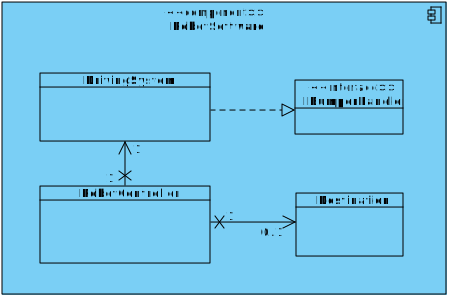
\includegraphics[width=1\textwidth]{img/52}
	\caption{Komponentendiagramm für den \emph{Robot}}
	\label{KomponentendiagrammKonkretRobot}
\end{figure}
In Abbildung \ref{KomponentendiagrammKonkretRobot} ist das konkrete Komponentendiagramm der \emph{Robot}-Komponente dargestellt. \emph{RobotSoftware} ist für die Steuerung der \textit{RobotUnit} zuständig. Die von der abstrakten Hardware 
des \textit{Robot} angebotenen, vorgegebenen Interfaces \textit{INorthStar, IBattery, IDrive, IDistanceSensors, IBumper} sowie 
\textit{IBumperHandler} werden dabei von der \textit{Robot}-Komponente für die konkrete Steuerung der \textit{RobotUnit} genutzt.
